%
\setcounter{table}{0}
\setcounter{figure}{0}
% the appendix no longer requires the prefix Appendix <Letter>
\chapter{Use cases (Detailed description)}%
\label{ch:append-UseCases}
In this section, the main use cases are described extensively. As many uses
cases are similar, only changing the parameter to which they refer to, the
Lighting subsystem was used as an example for the Manage<Parameter> use case,
where <Parameter> is Temperature, DoorBell, DateAndTime and SystemNotifications.

\begin{table}
  \captionsetup{justification=raggedright, singlelinecheck=false}
  \caption{Use case LoadGeometryFile}
  \centering
  \begin{tabular}{p{0.26\textwidth}p{0.64\textwidth}}
    \hline
    Use case name & \textbf{LoadGeometryFile} \\ \hline
     Participating actors      & Initiated by the User \\ \hline
     Flow of events & \begin{enum-c}
     \item The User selects the load geometry file option.
     \item The User selects the geometry file to load from a list.
     \item If the file is successfully loaded, the filename is displayed,
       and the file previewed (include \underline{PreviewGeometryFile} use
       case).
     \item Otherwise, an error message is displayed to the user.
     \end{enum-c}\\ \hline 
     Entry conditions       & The User has started the MMSLS machine control
     software and has previously generated a valid geometry file. \\ \hline 
      Exit conditions & The file is successfully loaded, previewed and with the
      filename displayed or an error message is displayed to the User.\\ \hline 
      Quality requirements &  Feedback must be given to the user within 2
      seconds; if files are ``heavy'', display an ongoing processing.\\ \hline 
  \end{tabular}%
\label{tab:us-load-geom}
\end{table}
%\setcounter{table}{0}
\setcounter{figure}{0}
% the appendix no longer requires the prefix Appendix <Letter>
\chapter{Use cases (Detailed description)}%
\label{ch:append-UseCases}
In this section, the main use cases are described extensively. As many uses
cases are similar, only changing the parameter to which they refer to, the
Lighting subsystem was used as an example for the Manage<Parameter> use case,
where <Parameter> is Temperature, DoorBell, DateAndTime and SystemNotifications.

\begin{table}
  \captionsetup{justification=raggedright, singlelinecheck=false}
  \caption{Use case LoadGeometryFile}
  \centering
  \begin{tabular}{p{0.26\textwidth}p{0.64\textwidth}}
    \hline
    Use case name & \textbf{LoadGeometryFile} \\ \hline
     Participating actors      & Initiated by the User \\ \hline
     Flow of events & \begin{enum-c}
     \item The User selects the load geometry file option.
     \item The User selects the geometry file to load from a list.
     \item If the file is successfully loaded, the filename is displayed,
       and the file previewed (include \underline{PreviewGeometryFile} use
       case).
     \item Otherwise, an error message is displayed to the user.
     \end{enum-c}\\ \hline 
     Entry conditions       & The User has started the MMSLS machine control
     software and has previously generated a valid geometry file. \\ \hline 
      Exit conditions & The file is successfully loaded, previewed and with the
      filename displayed or an error message is displayed to the User.\\ \hline 
      Quality requirements &  Feedback must be given to the user within 2
      seconds; if files are ``heavy'', display an ongoing processing.\\ \hline 
  \end{tabular}
\label{tab:us-load-geom}
\end{table}

\begin{table}
  \captionsetup{justification=raggedright, singlelinecheck=false}
  \caption{Use case PreviewGeometryFile}
  \centering
  \begin{tabular}{p{0.26\textwidth}p{0.64\textwidth}}
    \hline
    Use case name & \textbf{PreviewGeometryFile} \\ \hline
     Participating actors      & Initiated by the User \\ \hline
     Flow of events & \begin{enum-c}
     \item The User loads the geometry file.
     \item The geometry file is displayed on the canvas.
     \end{enum-c}\\ \hline 
     Entry conditions       & A valid geometry file is loaded into the
     application. \\ \hline 
      Exit conditions & The geometry file is displayed on canvas.      \\ \hline 
      Quality requirements & The preview should be resizable to accommodate
      the various component's dimensions. \\ \hline 
  \end{tabular}
\label{tab:us-prev-geom}
\end{table}

\begin{table}
  \captionsetup{justification=raggedright, singlelinecheck=false}
  \caption{Use case AssignColorsToLaserParams}
  \centering
  \begin{tabular}{p{0.26\textwidth}p{0.64\textwidth}}
    \hline
    Use case name & \textbf{AssignColorsToLaserParams} \\ \hline
     Participating actors      & Initiated by the User \\ \hline
     Flow of events & \begin{enum-c}
     \item The User selects a layer.
     \item The User associates a material's color to its laser's processing color
       counterpart.
     \item The User can edit the laser's processing color attributes.
     \end{enum-c}\\ \hline 
     Entry conditions       & The file is successfully loaded into the
     application and the preview is editable. \\ \hline 
      Exit conditions & The materials' colors has been assigned to valid laser's
      processing color with the respective processing parameters.\\ \hline 
      Quality requirements & Allow multiple line selection. \\ \hline 
  \end{tabular}
\label{tab:us-assign-colors}
\end{table}

\begin{table}
  \captionsetup{justification=raggedright, singlelinecheck=false}
  \caption{Use case LoadManufFile}
  \centering
  \begin{tabular}{p{0.26\textwidth}p{0.64\textwidth}}
    \hline
    Use case name & \textbf{LoadManufFile} \\ \hline
     Participating actors      & Initiated by the User \\ \hline
     Flow of events & \begin{enum-c}
     \item The User selects the load manufacturing file option.
     \item The User selects the manufacturing file to load from a list.
     \item If the file is successfully loaded, the filename is displayed.
     \item Otherwise, an error message is displayed to The User.
     \end{enum-c}\\ \hline 
     Entry conditions       & The User has started the MMSLS machine control
     software and has previously generated a valid manufacturing file. \\ \hline 
      Exit conditions & The file is successfully loaded and with the
      filename displayed or an error message is displayed to the User.      \\ \hline 
      Quality requirements & Feedback must be given to the user within 2
      seconds; if files are 'heavy', display an ongoing processing. \\ \hline 
  \end{tabular}
\label{tab:us-load-manuf}
\end{table}

\begin{table}
  \captionsetup{justification=raggedright, singlelinecheck=false}
  \caption{Use case ConnectToMach}
  \centering
  \begin{tabular}{p{0.26\textwidth}p{0.64\textwidth}}
    \hline
    Use case name & \textbf{ConnectToMach} \\ \hline
     Participating actors      & Initiated by the User \\ \hline
     Flow of events & \begin{enum-c}
     \item The User selects the appropriate connection to the machine from a list.
     \item The User selects the \emph{Connect to Machine} option.
     \item If the connection is successful, the connection status is updated to
       \emph{Connected} and machine operation options are enabled.
     \item Otherwise, an error message is displayed to The User.
     \end{enum-c}\\ \hline 
     Entry conditions       & The User has started the MMSLS machine control
     software and there is physical connection between the \emph{Master} system and
     the \gls{mms}  machine. \\ \hline 
      Exit conditions & The connection is established between \emph{Master} system and
      the \gls{mms} machine or an error message is displayed to the user.\\ \hline 
  \end{tabular}
\label{tab:us-con-to-mach}
\end{table}

\begin{table}
  \captionsetup{justification=raggedright, singlelinecheck=false}
  \caption{Use case DisconnectToMach}
  \centering
  \begin{tabular}{p{0.26\textwidth}p{0.64\textwidth}}
    \hline
    Use case name & \textbf{DisconnectToMach} \\ \hline
     Participating actors      & Initiated by the User \\ \hline
     Flow of events & \begin{enum-c}
     \item The User selects the \emph{Disconnect to Machine} option.
     \item If the disconnection is successful, the connection status is updated to
       \emph{Disconnected} and machine operation options are disabled.
     \item Otherwise, an error message is displayed to The User.
     \end{enum-c}\\ \hline 
     Entry conditions       & A successful connection between the \emph{Master} system
     and the \gls{mms} machine is established.\\ \hline 
      Exit conditions & The connection is closed and the machine operations
      options are disabled or an error messaged is displayed to the user \\ \hline 
  \end{tabular}
\label{tab:us-discon-to-mach}
\end{table}

\begin{table}
  \captionsetup{justification=raggedright, singlelinecheck=false}
  \caption{Use case ManualResetMach}
  \centering
  \begin{tabular}{p{0.26\textwidth}p{0.64\textwidth}}
    \hline
    Use case name & \textbf{ManualResetMach} \\ \hline
     Participating actors      & Initiated by the User \\ \hline
     Flow of events & \begin{enum-c}
     \item The User selects the axis to reset, the direction and the reset
       distance.
     \item When the reset is satisfactory, The User acknowledges this fact by
       selecting the option \emph{Reset end}.
     \item The option to \emph{Start Manufacturing} is now enabled.
     \end{enum-c}\\ \hline 
     Entry conditions       &  A successful connection between the \emph{Master}
     system and the \gls{mms} machine is established.\\ \hline 
      Exit conditions & The reset is satisfactory (User has selected option
      \emph{Reset End}) and the \emph{Start Manufacturing} is enabled.      \\ \hline 
      Quality requirements & Provide feedback to the User of the manual reset
      operations (ascent/descent of the axis) \\ \hline 
  \end{tabular}
\label{tab:us-man-reset}
\end{table}

\begin{table}
  \captionsetup{justification=raggedright, singlelinecheck=false}
  \caption{Use case StartManuf}
  \centering
  \begin{tabular}{p{0.26\textwidth}p{0.64\textwidth}}
    \hline
    Use case name & \textbf{StartManuf} \\ \hline
     Participating actors      & Initiated by the user \\ \hline
     Flow of events & \begin{enum-c}
     \item The User selects the \emph{Start manufacturing} option.
     \item If successful, the machine initiates the manufacturing process
       the machine status is updated to \emph{Run}.
     \end{enum-c}\\ \hline 
     Entry conditions       & \begin{enum-c}
     \item A successful connection between the \emph{Master} system
     and the \gls{mms} machine is established. 
      \item Reset is finished.
      \item Valid geometry and manufacturing file have been loaded.
     \end{enum-c}\\ \hline 
      Exit conditions & \begin{item-c}
      \item \emph{Success}: The \gls{mms} machine status is updated to \emph{Run}, the
        \emph{Start manufacturing} option is disabled, and the options
       \emph{Pause manufacturing} and \emph{Stop manufacturing} are enabled.
     \item \emph{Fail}: An error message is displayed to the user.
      \end{item-c}\\ \hline
      Quality requirements & Update the relevant processing information to the
        User (include use case \underline{UpdateInfo}). \\ \hline 
  \end{tabular}
\label{tab:us-start-manuf}
\end{table}

\begin{table}
  \captionsetup{justification=raggedright, singlelinecheck=false}
  \caption{Use case PauseManuf}
  \centering
  \begin{tabular}{p{0.26\textwidth}p{0.64\textwidth}}
    \hline
    Use case name & \textbf{PauseManuf} \\ \hline
     Participating actors      & Initiated by the user \\ \hline
     Flow of events & \begin{enum-c}
     \item The User selects the \emph{Pause manufacturing} option.
     \item If successful, the manufacturing process is paused.
     \end{enum-c}\\ \hline 
     Entry conditions       & The manufacturing has started (startManuf was
     triggered), but has not yet finished. \\ \hline 
      Exit conditions & \begin{item-c}
      \item \emph{Success}: The manufacturing process is paused, and
        the \gls{mms} machine status is updated to \emph{Idle}. The \emph{Pause
        manufacturing} option is disabled and the \emph{Start manufacturing}
        option is re-enabled.
     \item \emph{Fail}: An error message is displayed to the user.
      \end{item-c}\\ \hline
  \end{tabular}
\label{tab:us-pause-manuf}
\end{table}

\begin{table}
  \captionsetup{justification=raggedright, singlelinecheck=false}
  \caption{Use case StopManuf}
  \centering
  \begin{tabular}{p{0.26\textwidth}p{0.64\textwidth}}
    \hline
    Use case name & \textbf{StopManuf} \\ \hline
     Participating actors      & Initiated by the User \\ \hline
     Flow of events & \begin{enum-c}
     \item The User selects the \emph{Stop manufacturing} option.
     \item If successful, the manufacturing process is stopped.
     \end{enum-c}\\ \hline 
     Entry conditions & The manufacturing has started (startManuf was
     triggered), but has not yet finished. \\ \hline 
      Exit conditions & \begin{item-c}
      \item \emph{Success}: The manufacturing process is stopped, and
        the \gls{mms} machine status is updated to \emph{Stopped}. The
        \emph{Stop manufacturing} option is disabled and the \emph{Start
        manufacturing} option is re-enabled.
     \item \emph{Fail}: An error message is displayed to the user.
      \end{item-c}\\ \hline
  \end{tabular}
\label{tab:us-stop-manuf}
\end{table}

Although several notifications from relevant events are to be notified by the
\emph{Master} machine to the User, for brevity purposes only the most relevant one is
showcased here, namely \underline{NotifyManufEnd}.

\begin{table}
  \captionsetup{justification=raggedright, singlelinecheck=false}
  \caption{Use case NotifyManufEnd}
  \centering
  \begin{tabular}{p{0.26\textwidth}p{0.64\textwidth}}
    \hline
    Use case name & \textbf{NotifyManufEnd} \\ \hline
     Participating actors      & Initiated by MMS-Mach; User participates \\ \hline
     Flow of events & \begin{enum-c}
     \item When manufacturing is completed, the \emph{Master} system notifies The User
       about this fact.
     \end{enum-c}\\ \hline 
     Entry conditions & The manufacturing has started (startManuf was
     triggered), and is not paused or stopped. \\ \hline 
     Exit conditions & The manufacturing process stops and the User is notified
      about this fact.\\ \hline 
  \end{tabular}
\label{tab:us-notif-manuf-end}
\end{table}

\begin{table}[!hbt]
  \captionsetup{justification=raggedright, singlelinecheck=false}
  \caption{Use case VisualizeManuf}
  \centering
  \begin{tabular}{p{0.26\textwidth}p{0.64\textwidth}}
    \hline
    Use case name & \textbf{VisualizeManuf} \\ \hline
     Participating actors      & Initiated by MMS-Mach or Laser; User participates \\ \hline
     Flow of events & \begin{enum-c}
     \item Relevant manufacturing information is sent by the MMS-Mach or the
       Laser to the \emph{Master} system --- on a time-basis or triggered by a
       relevant event like the manufacturing completion of one layer --- that is
       updated to the User.
     \end{enum-c}\\ \hline 
     Entry conditions & The manufacturing has started (startManuf was
     triggered)\\ \hline
      Exit conditions & The manufacturing is stopped or has ended. \\ \hline 
      Quality requirements & \begin{item-c}
      \item \emph{Time-basis} The relevant manufacturing information must be
        updated with 1 second refresh rate.
      \item \emph{Event} The information associated with the triggering event
        must be updated immediately.
      \end{item-c} \\ \hline 
  \end{tabular}
\label{tab:vis-manuf}
\end{table}

%%% Local Variables:
%%% mode: latex
%%% TeX-master: "../../dissertation"
%%% End:

%\setcounter{table}{0}
\setcounter{figure}{0}
%
\chapter{Sequence Diagrams}
\label{ch:append-seq-diag}
\begin{figure*}
  \begin{center}
    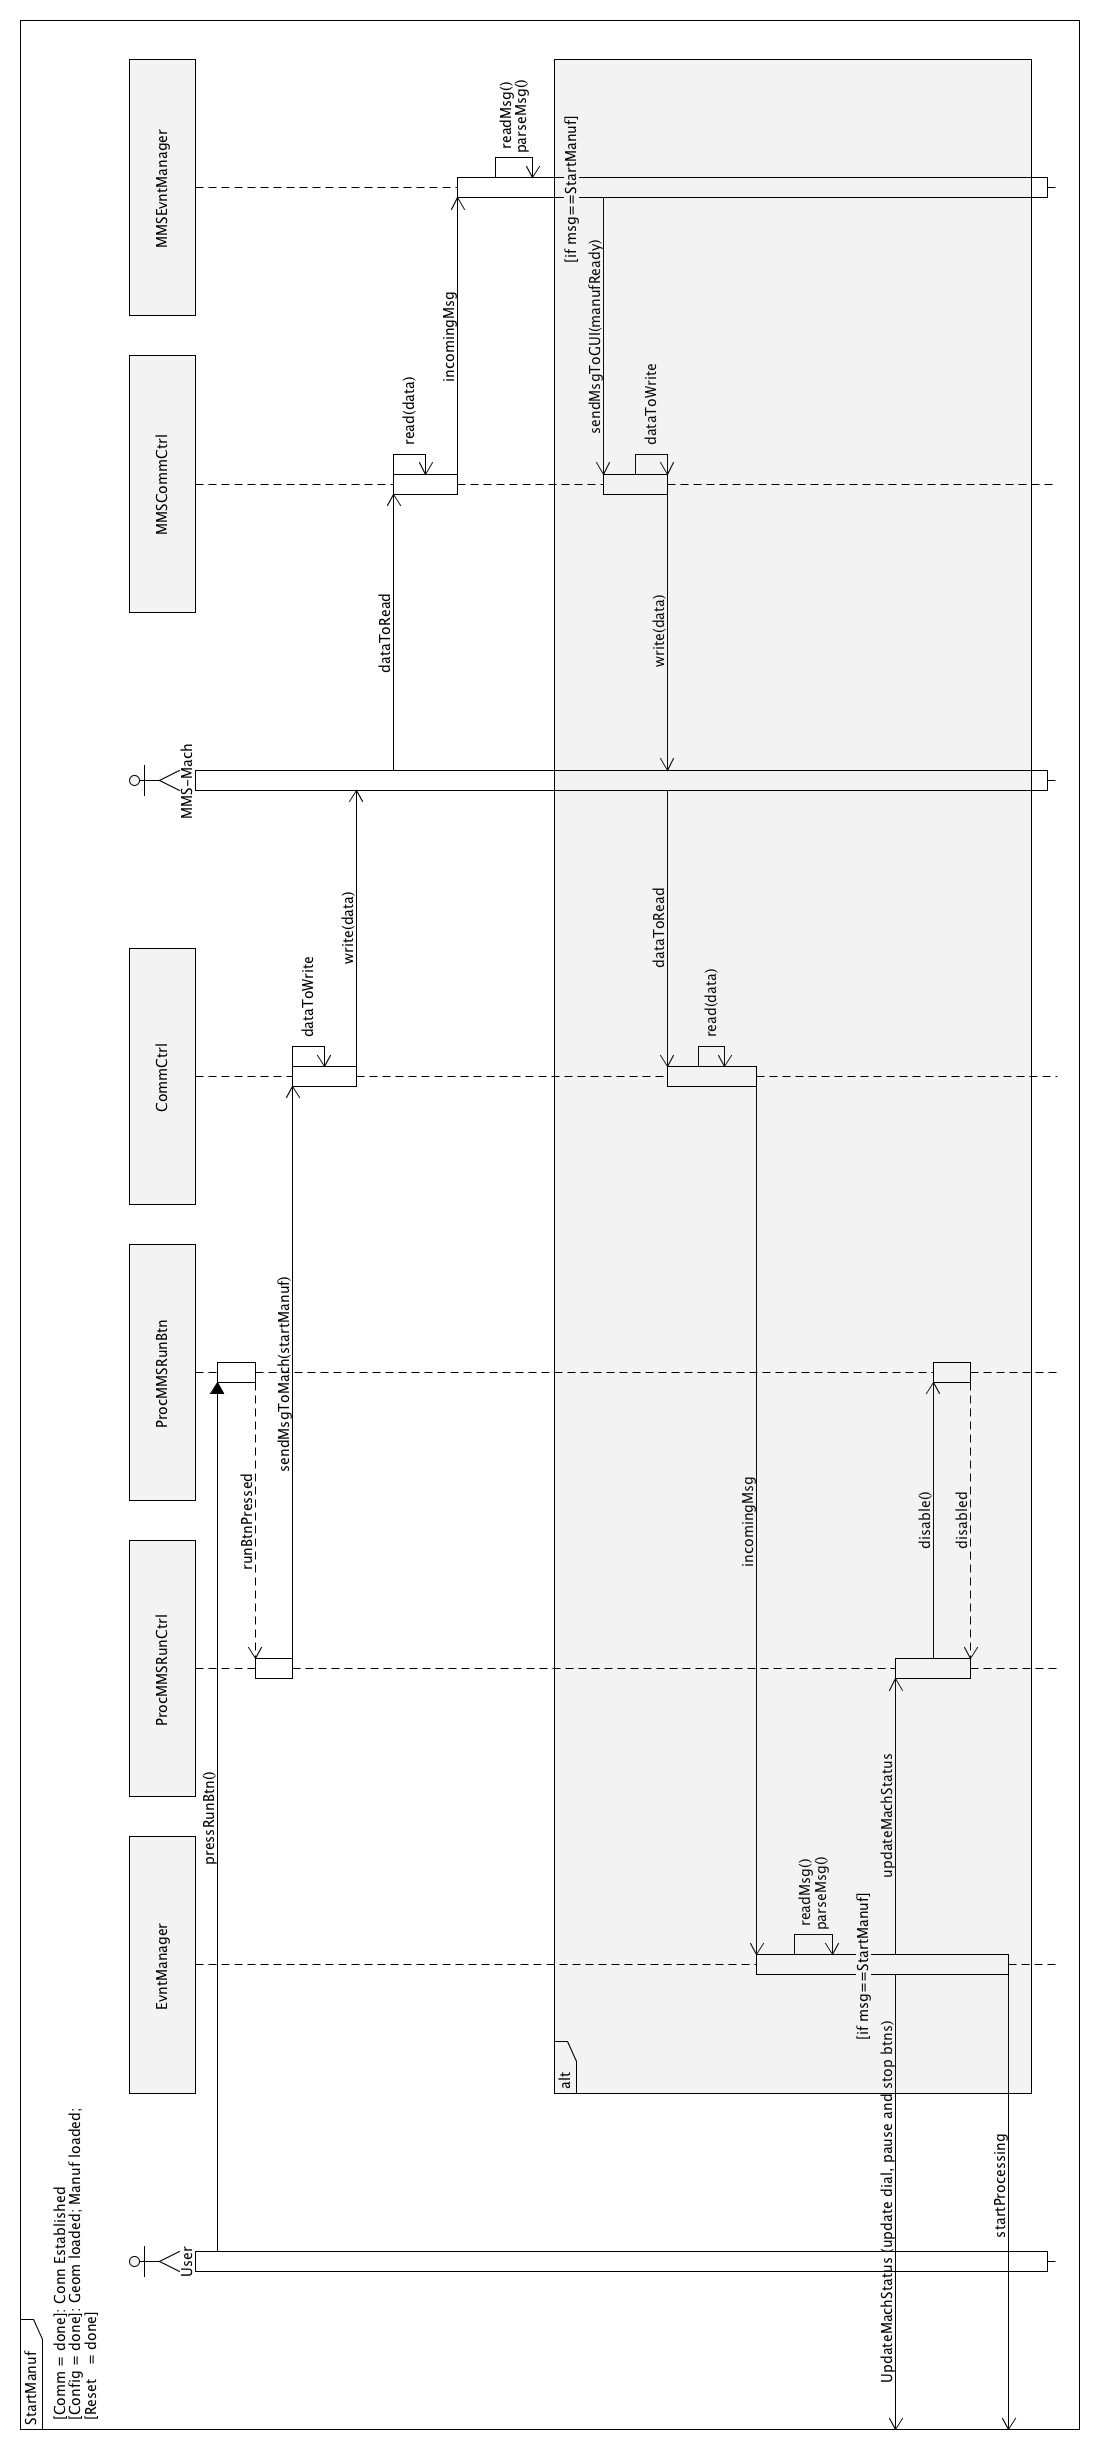
\includegraphics[height=1.0\textheight]{./img/seq-start-manuf-lscape.png}
  \end{center}
  \caption{Sequence diagram for the \emph{StartManuf} use case (Part 1)}\label{fig:seq-start-manuf-lscape}
\end{figure*}

\begin{figure*}
  \begin{center}
    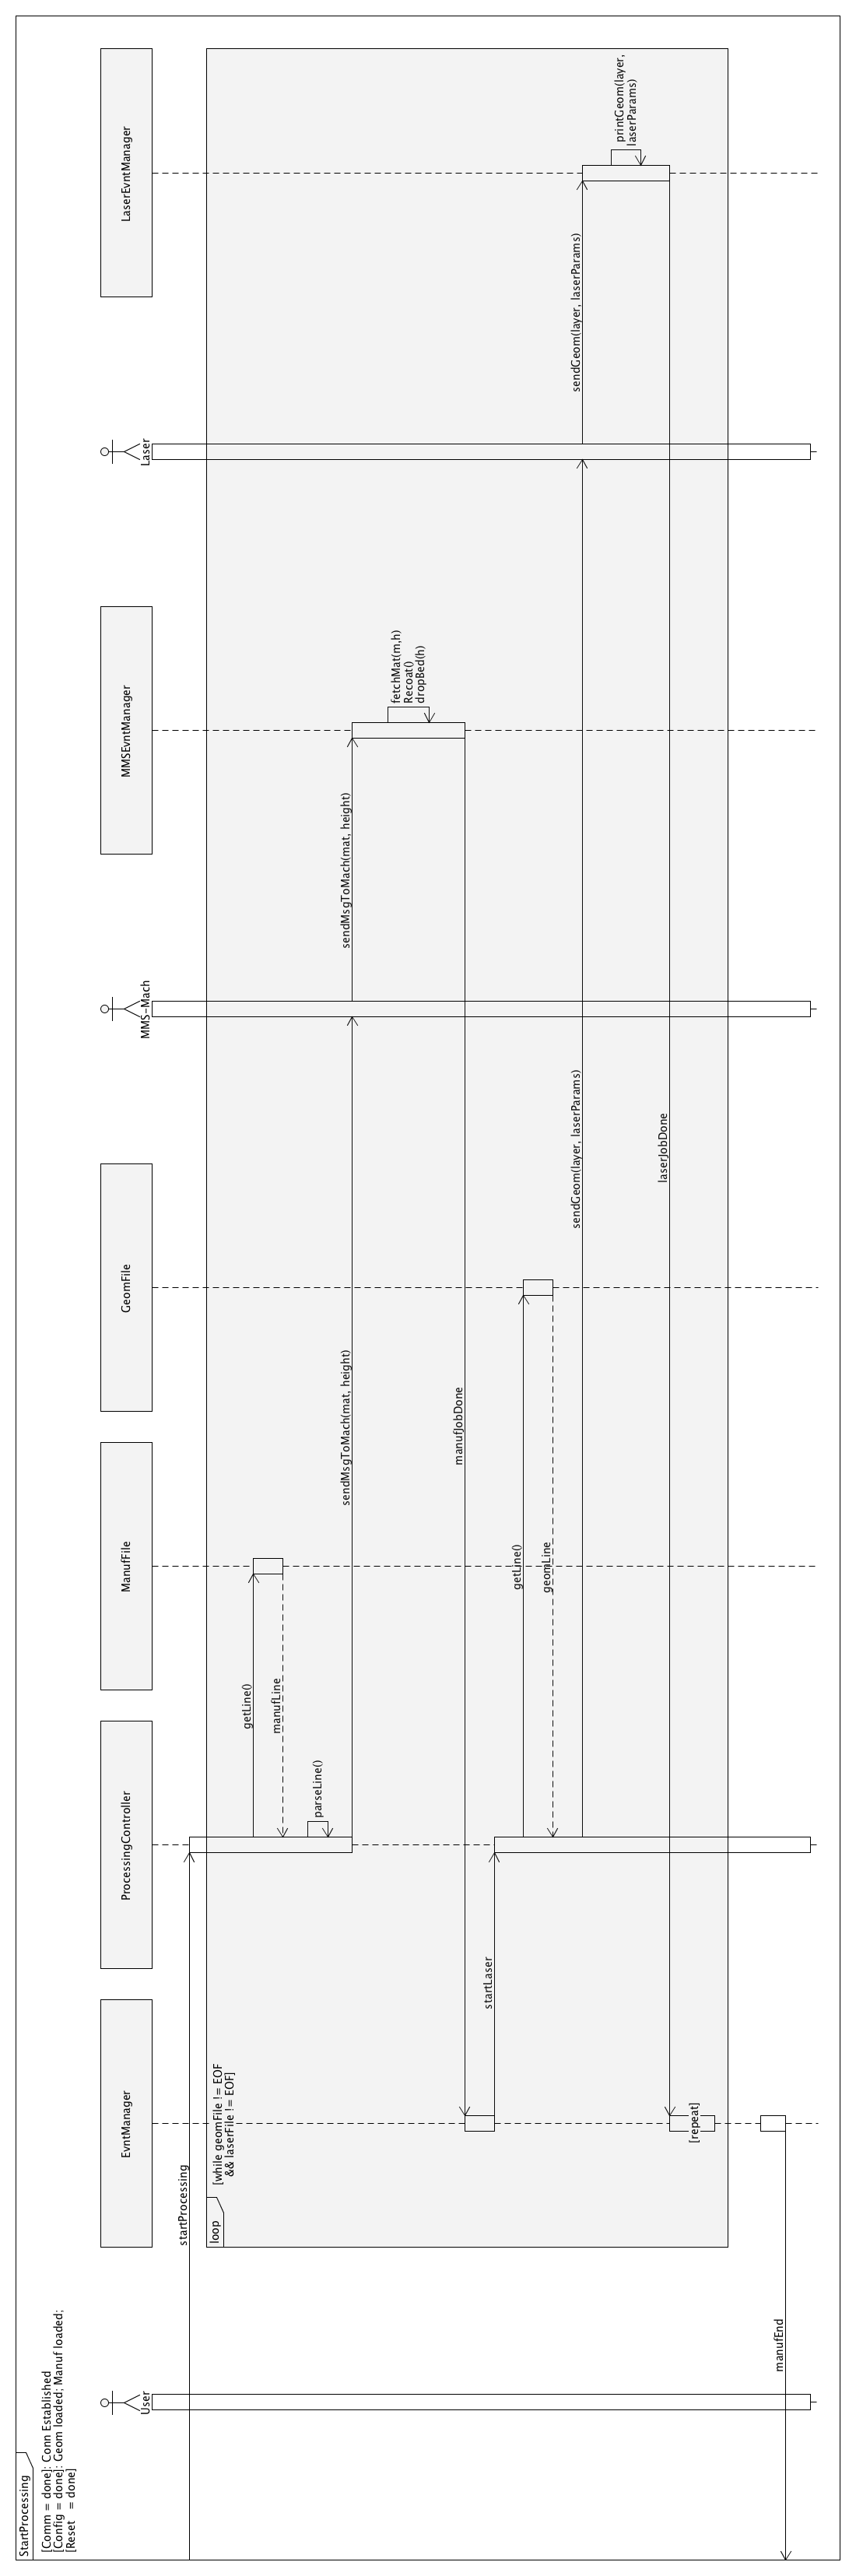
\includegraphics[height=1.0\textheight]{./img/seq-start-process-lscape.png}
  \end{center}
  \caption{Sequence diagram for the \emph{StartManuf} use case (Part 2)}\label{fig:seq-start-process-lscape}
\end{figure*}
%
%\clearpage
%
%% src:https://www.reddit.com/r/LaTeX/comments/4jynr7/adding_a3_pdf_page_into_an_a4_document/d3ba7eg/ 
%\KOMAoptions{paper=A3,pagesize}
%%\KOMAoptions{paper=landscape, pagesize}
%
%\label{ch:append-UseCases}
%\begin{figure*}
%  \begin{center}
%    \includegraphics[width=1.6\textwidth]{./img/seq-start-manuf.png}
%  \end{center}
%  \caption{Sequence diagram for the \emph{StartManuf} use case (Part 1)}%
%\label{fig:seq-start-manufA3}
%\end{figure*}
%
%\begin{figure*}
%  \begin{center}
%    \includegraphics[width=1.6\textwidth]{./img/seq-start-process.png}
%  \end{center}
%  \caption{Sequence diagram for the \emph{StartManuf} use case (Part 2)}%
%\label{fig:seq-start-processA3}
%\end{figure*}
%
%\cleardoublepage
%\KOMAoptions{paper=A4, pagesize}

%%% Local Variables:
%%% mode: latex
%%% TeX-master: "Report"
%%% End:
